%%%%%%%%%%%%%%%%%%%%%%%%%%%%%%%%%
% This is a slightly modified template of the one built by
% Steven V. Miller. Information can be found here:
%  http://svmiller.com/blog/2016/02/svm-r-markdown-manuscript/
%
% I added in a few other features.
%
% Here are the options that you can define in the YAML
% header.
%
% fontfamily - self-explanatory
% fontsize - self-explanatory (e.g. 10pt, 11pt)
% anonymous - true/false. If true, names will be supressed and the
%                       text will be double-spaced and ragged
%                       right with a separate page for title and abstract.
% endnotes - true/false. If true, the footnotes will be put in a
%                   section at the end just ahead of the references.
% endfloat - move all tables and figures to the end of the document
% keywords - self-explanatory
% thanks - shows up as a footnote to the title on page 1
% abstract - self explanatory
% appendix - if true, tables and figures will have  in
%                   front
% appendixletter - The letter to append to tables and figures in
%                             appendix
% pagenumber - Put in a number here to get a starting page number
%                         besides 1.
%%%%%%%%%%%%%%%%%%%%%%%%%%%%%%%%%%


\documentclass[11pt,]{article}
\usepackage[left=1in,top=1in,right=1in,bottom=1in]{geometry}
\usepackage{amsmath}
\usepackage{float}
\usepackage{dcolumn}
\usepackage{graphicx}

\newcommand*{\authorfont}{\fontfamily{phv}\selectfont}
\usepackage[]{mathpazo}


\usepackage[T1]{fontenc}
\usepackage[utf8]{inputenc}

\usepackage{abstract}
\renewcommand{\abstractname}{}    % clear the title
\renewcommand{\absnamepos}{empty} % originally center

\providecommand{\tightlist}{%
  \setlength{\itemsep}{0pt}\setlength{\parskip}{0pt}}

\renewenvironment{abstract}
 {{%
    \setlength{\leftmargin}{0mm}
    \setlength{\rightmargin}{\leftmargin}%
  }%
  \relax}
 {\endlist}

\makeatletter
\def\@maketitle{%
  \newpage
%  \null
%  \vskip 2em%
%  \begin{center}%
  \let \footnote \thanks
    {\fontsize{18}{20}\selectfont\raggedright  \setlength{\parindent}{0pt} \@title \par}%
}
%\fi
\makeatother




\setcounter{secnumdepth}{0}

\usepackage{longtable,booktabs}

\title{Patterns of Panethnic Intermarriage in the United States, 1980-2018  }



\author{\Large Aaron Gullickson\vspace{0.05in} \newline\normalsize\emph{University of Oregon, Sociology}  }


\date{}

\usepackage{titlesec}

\titleformat*{\section}{\normalsize\bfseries}
\titleformat*{\subsection}{\normalsize\itshape}
\titleformat*{\subsubsection}{\normalsize\itshape}
\titleformat*{\paragraph}{\normalsize\itshape}
\titleformat*{\subparagraph}{\normalsize\itshape}


\usepackage{natbib}
\setcitestyle{aysep={}}
\bibliographystyle{./resources/ajs.bst}


%packages needed by kableExtra
\usepackage{booktabs}
\usepackage{longtable}
\usepackage{array}
\usepackage{multirow}
\usepackage{wrapfig}
\usepackage{float}
\usepackage{colortbl}
\usepackage{pdflscape}
\usepackage{tabu}
\usepackage{threeparttable}
\usepackage{threeparttablex}
\usepackage[normalem]{ulem}
\usepackage{makecell}
\usepackage{xcolor}

%\renewcommand{\refname}{References}
%\makeatletter
%\renewcommand\bibsection{
%    \section*{{\normalsize{\refname}}}%
%}%
%\makeatother

\newtheorem{hypothesis}{Hypothesis}
\usepackage{setspace}

\makeatletter
\@ifpackageloaded{hyperref}{}{%
\ifxetex
  \usepackage[setpagesize=false, % page size defined by xetex
              unicode=false, % unicode breaks when used with xetex
              xetex]{hyperref}
\else
  \usepackage[unicode=true]{hyperref}
\fi
}
\@ifpackageloaded{color}{
    \PassOptionsToPackage{usenames,dvipsnames}{color}
}{%
    \usepackage[usenames,dvipsnames]{color}
}
\makeatother
\hypersetup{breaklinks=true,
            bookmarks=true,
            pdfauthor={},
             pdfkeywords = {panethnicity; intermarriage; assortative mating, ethnic exogamy; immigration},
            pdftitle={Patterns of Panethnic Intermarriage in the United States, 1980-2018},
            colorlinks=true,
            citecolor=blue,
            urlcolor=blue,
            linkcolor=magenta,
            pdfborder={0 0 0}}
\urlstyle{same}  % don't use monospace font for urls

\usepackage{endnotes}


  \usepackage[notablist,nofiglist,noheads,tablesfirst]{endfloat}

\newlength{\normalparindent}
\setlength{\normalparindent}{\parindent}

%prettier captions for figures and tables
%I am making the text of figure captions smaller but not table captions
\usepackage[labelfont=bf,labelsep=period]{caption}
\captionsetup[figure]{font=footnotesize}

\begin{document}

% \pagenumbering{arabic}% resets `page` counter to 1
%


%\pagenumbering{gobble}

% \maketitle

{% \usefont{T1}{pnc}{m}{n}
\setlength{\parindent}{0pt}
\thispagestyle{plain}
{\fontsize{18}{20}\selectfont\raggedright
\maketitle  % title \par

}

{
   \vskip 13.5pt\relax \normalsize\fontsize{11}{12}
\hfill 

}

}







\begin{abstract}

    \hbox{\vrule height .2pt width 39.14pc}

    \vskip 8.5pt % \small

\noindent Intermarriage among ethnic groups belonging to the same panethnic category (e.g.~Asian, Latino) is an important indicator of the strength of panethnicity. Yet, most of the work on panethnic intermarriage uses older samples with significant data limitations. In this article, I use data on recently married couples from the American Community Survey 2014-18 and Census 1980 to analyze the likelihood of ethnic exogamy within the panethnic categories of Latino, East/Southeast Asian, and South Asian. I utilize a counterfactual marriage model that accounts for group size within local marriage markets, eliminates immigrants married abroad from analysis, and controls for birthplace and language endogamy. The results show that birthplace and language diversity are significant barriers to ethnic exogamy among Asians but not Latinos. Once birthplace and language endogamy are held constant, panethnic intermarriage is far more likely among Asians than among Latinos. East/Southeast Asian ethnic exogamy has increased over time, while Latino ethnic exogamy has not. Furthermore, East/Southeast Asian and South Asian intermarriage remains rare, suggesting that panethnic intermarriage among Asians occurs within two separate melting pots.


\vskip 8.5pt \noindent \emph{Keywords}: panethnicity; intermarriage; assortative mating, ethnic exogamy; immigration \par

    \hbox{\vrule height .2pt width 39.14pc}



\end{abstract}


\vskip 6.5pt

\noindent \newpage\doublespacing\raggedright\setlength{\parindent}{\normalparindent} \hypertarget{introduction}{%
\section{Introduction}\label{introduction}}

Social scientists treat intermarriage as a prime indicator of the strength of social boundaries separating groups \citep{gordon_assimilation_1964}. While an increase in intermarriage across one boundary typically indicates that the given boundary is weakening, it can also signify a reshaping and strengthening of broader group identities. For example, widespread intermarriage among European ethnic groups in the mid-twentieth century contributed to the breakdown of salient ethnic divisions between these populations but also helped to re-consolidate a sense of collective whiteness \citep{lieberson_many_1988, alba_ethnic_1990, jacobsen_whiteness_1998}. Similarly, intermarriage is seen as a key benchmark to gauge panethnic affinity among Asian and Latino ethnic groups today.

Panethnicity is defined by \citet{okamoto_panethnicity_2014a} as ``the construction of a new categorical boundary through the consolidation of ethnic, tribal, religious, or national groups.'' Within the literature on ethnoracial boundary formation, panethnicity is treated as a form of boundary expansion in which the salient boundary shifts from a lower to a higher level within a nested hierarchy of possible identification \citep{wimmer_making_2008}.\footnote{For analytical clarity, I use the term ``ethnoracial'' to refer to any group that may be identified either along racial or ethnic lines in popular practice, ``racial group'' to refer to the five major groups of White, Black, Indigenous, Asian, and Latino that constitute the highest level in the nested hierarchy of ethnoracial differences, and ``ethnic group'' to refer to different sub-populations among Asians and Latinos that are primarily defined in terms of national origin, such as Chinese, Korean, Mexican, and Colombian. Ethnic differentiation within the same national origin group exists as well, but is largely unmeasurable in the data that I use here.} From this perspective, ethnoracial categories are not fixed and stable, but rather can shift over time, as they have for the ethnoracial groups in the US that we now collectively view as White and Black. Understanding these processes for contemporary Asian and Latino ethnic groups informs us about how social boundaries might shift in the future. Such shifts are consequential for issues of racial inequality, assimilation, political change, and even how we measure race and ethnicity.

Scholars have long recognized the importance of understanding ``interpersonal'' panethnicity in the form of affinity for panethnic marriage partners \citep[pp.~167-168]{espiritu_asian_1993}. Early attempts used simple outmarriage percentages which generally show the effects of group size more than underlying affinity \citep{shinagawa_asian_1996}. However, shortly after the turn of the century, several more sophisticated studies examined panethnic intermarriage among Asian and Latino ethnic groups \citep{qian_asian_2001, rosenfeld_salience_2001, qian_latinos_2004, fu_how_2007a, qian_crossing_2012}. This work found substantial evidence of panethnic intermarriage among East/Southeast Asian ethnic groups, but produced less consistent and contrary findings regarding the strength of panethnic intermarriage among Latinos.

Despite the important contributions of this prior work, our existing understanding of panethnic intermarriage is substantially out of date. Prior research primarily used data from Census 1980, 1990, or 2000 and much of this work relied upon an examination of panethnicity among the relatively few Asian and Latino groups numerically large enough in historical data to sustain an analysis. Notably, South Asian ethnic groups were excluded from most prior research, despite active interest among panethnic scholars in the degree to which Asian panethnicity incorporates South Asians \citep{kibria_not_1996}. Newer data and methodologies offer an opportunity to update and expand our understanding of both the prevalence and heterogeneity in panethnic intermarriage across a wider selection of Asian and Latino ethnic groups. The increasing diversity of the US population, primarily driven by Asian and Latino population growth further motivates the need to return to this topic.

In this article, I measure the frequency of panethnic intermarriage in recent data from the 2014-2018 American Community Survey using a modeling approach that allows me to improve on limitations in prior work and to ask novel research questions. Additionally, I conduct a parallel analysis of Census 1980 data to provide a measure of the change in panethnic intermarriage over time. Specifically, my research is guided by the following questions:

\begin{enumerate}
\def\labelenumi{\arabic{enumi}.}
\tightlist
\item
  How common is panethnic intermarriage among East/Southeast Asian, South Asian, and Latino ethnic groups today, in comparison to interracial marriage?
\item
  Has panethnic intermarriage become more common over time?
\item
  How heterogeneous is panethnic intermarriage across combinations of specific Asian and Latino ethnic groups?
\item
  How does birthplace and language endogamy effect our measures of panethnic intermarriage?
\end{enumerate}

To address these research questions, I use a conditional logit model approach \citep{gullickson_counterfactual_2021} that allows me to easily adjust for differences in the size and spatial distribution of ethnoracial groups and to include a variety of other variables that may present structural barriers to panethnic intermarriage. I use this model to specifically account for the role of birthplace and language endogamy. The considerable diversity in birthplace and language both within and between Asian and Latino ethnic groups plays a complex role in panethnic intermarriage. Researchers has largely tried to address this issue indirectly by including an immigrant-native comparison, but this comparison does not adequately capture the underlying complexity.

My findings help resolve existing disagreements in prior work on panethnic intermarriage, and extend this work in important ways. I find that birthplace and language endogamy present substantial barriers to panethnic intermarriage among Asians but not Latinos. After accounting for these barriers, I find significant differences in the relative frequency, trends, and heterogeneity of Asian and Latino panethnic intermarriage. These findings have important implications for our understanding of panethnicity more broadly and the future of existing ethnoracial boundaries.

\hypertarget{panethnicity-in-marriage}{%
\section{Panethnicity in Marriage}\label{panethnicity-in-marriage}}

Scholars of panethnic intermarriage have focused on several related research questions. First, researchers have attempted to assess the strength of panethnic intermarriage by comparing its likelihood to that of interracial outmarriage. Prior work consistently finds that Asian panethnic intermarriage is more likely than interracial outmarriage, while the results for Latinos are less consistent. Using data from Census 1990, \citet{qian_asian_2001} found Asian panethnic intermarriage to be more common than intermarriage with Whites, although the degree of difference varied by the specific Asian ethnic group. \citet{fu_how_2007a} examined native-born couples from the same data source and similarly found Asian panethnic intermarriage to be substantially more likely than Asian outmarriage with Whites, Blacks, and Latinos. \citet{fu_how_2007a} also found Latino panethnic intermarriage to be slightly less likely than outmarriage with Whites but more likely than outmarriage with Blacks and Asians, it was slightly less likely than outmarriage with Whites. \citet{rosenfeld_salience_2001} used Census 1980 and 1990 data to examine Asian and Latino panethnic intermarriage in select US cities. The results vary across cities, but generally suggest that panethnic intermarriage is more likely than outmarriage with Whites and Blacks for both Asians and Latinos. \citet{qian_latinos_2004} used Census 1990 data to examine intermarriage between Mexicans, Puerto Ricans, and Cubans, as well as outmarriage to non-Latino Whites and Blacks. Their results varied across ethnic combinations and by the reported race of the Latino respondent, but they generally found relatively low rates of Latino panethnic intermarriage and little evidence that Latino panethnic intermarriage was consistently more common than outmarriage with Whites and Blacks. \citet{qian_crossing_2012} use slightly more recent Census 2000 data to examine panethnicity among Chinese, Filipino, Mexican, and Puerto Rican respondents. They found panethnic intermarriage to be substantially more likely for all four groups than outmarriage with either Whites or non-Whites.

Second, scholars have focused on comparing the relative strength of panethnicity between Latinos and Asians, which can clarify the weight of cultural and structural factors on panethnic intermarriage \citep{lopez_panethnicity_1990}. Cultural factors such as shared language and religion create affinity across ethnic boundaries. Structural factors such as economic and occupational similarity, spatial proximity, and the degree of racialization (the tendency of outsiders to treat all members of the panethnic category as a monolithic racial group) may also affect panethnic affinity. Latinos share cultural features such as language and religion that should promote panethnicity while Asians generally do not. On the other hand, racialization of Asians as a singular group tends to be stronger than for Latinos, who have an enduring history of racial ambiguity in the US \citep{lopez_panethnicity_1990, kibria_construction_1997, rodriguez_changing_2000a, fox_defining_2013}.

Both \citet{rosenfeld_salience_2001} and \citet{fu_how_2007a} found stronger patterns of panethnicity among Asians than Latinos, suggesting that structural factors such as racialization are more important in determining patterns of panethnic intermarriage than cultural factors. In contrast, \citet{qian_crossing_2012} found relative similar odds of panethnic intermarriage among their Mexican, Puerto Rican, Chinese, and Filipino respondents. Thus, prior research is somewhat inconsistent regarding the relative strength of panethnicity between Asians and Latinos, some of which may reflect different data sources, selection criteria, and methodology.

Third, prior work has explored the degree of heterogeneity in panethnic intermarriage among specific ethnic groups within a given panethnic category. Because of the degree to which studies vary in terms of the ethnic groups they include, this work is difficult to summarize succinctly, but one specific pattern is notable. Chinese/Japanese intermarriage is particularly common \citep{qian_asian_2001, rosenfeld_salience_2001}. This finding may reflect the fact that these two Asian groups have a longer history of US residence, but could also reflect an underlying regional distinction between East Asians and other Asian groups. However, the limited number of ethnic groups used in prior work makes it difficult to determine the importance of regional differences.

South Asian ethnic groups are notably absent from most prior work, owing in part to a small sample size in historical data sources. \citet{qian_asian_2001} do include an ``Asian Indian'' ethnic group and find no evidence of panethnic intermarriage between this group and other East/Southeast Asian ethnic groups. This finding is consistent with other research showing that in everyday practice South Asians are not treated as Asian in the US but rather as ``ambiguous non-whites'' \citep{kibria_not_1996, morning_racial_2001, schachter_finding_2014}. More recent work by \citet{lichter_whom_2015a} also shows low rates of outmarriage to other (non-South) Asian groups among Indian immigrants. However, due to sample size limitations, Asian Indians are the only South Asian population included in prior analyses, making it impossible to determine the extent of panethnicity among South Asian ethnic groups themselves.

Finally, prior work has explored the degree to which nativity affects the likelihood of panethnic intermarriage. Framed around assimilation theory, scholars argue that nativity may facilitate panethnic intermarriage and offer an alternative mode of assimilation \citep[p.~673]{qian_crossing_2012}. Rather than assimilate through interracial marriage with Whites, Asian and Latino ethnic groups may assimilate into larger panethnic identities. However, prior work is divided on the role of nativity in patterns of panethnic intermarriage. \citet{rosenfeld_salience_2001} found that that the odds of panethnic intermarriage increased among native-born Asians relative to their foreign-born counterparts, but decreased for native-born Latinos. \citet{qian_asian_2001} found similar results for Asians, but do not offer a comparison to Latinos. In contrast, \citet{qian_crossing_2012} found that the odds of panethnic intermarriage increased for natives and those immigrants who came to the US at an earlier age for all four Latino and Asian groups they studied.

Some of these discrepancies regarding nativity reflect a shortcoming in understanding the complex manner in which immigration and assimilation may affect patterns of panethnic intermarriage. In particular, comparisons between natives and immigrants fail to fully capture the ways that birthplace and language endogamy may present barriers to panethnic intermarriage. In the section that follows, I develop this argument more fully.

\hypertarget{the-role-of-birthplace-and-language-endogamy}{%
\subsection{The Role of Birthplace and Language Endogamy}\label{the-role-of-birthplace-and-language-endogamy}}

Individuals often prefer partners from the same birthplace due to the shared cultural understandings that arise from being born and raised in a particular place. Similarly, people are more likely to marry individuals who speak the same primary language. We might expect birthplace endogamy to lower the likelihood of panethnicity for both Asians and Latinos, because all Asian and Latino ethnic groups have a substantial foreign-born sub-population and these members would prefer to marry someone from the same place of birth. On the other hand, language endogamy might affect Asian and Latino panethnic intermarriage differently, because Latino ethnic groups share a common language while Asian ethnic groups do not.

However, the actual effect of birthplace and language endogamy on panethnic intermarriage is considerably more complex, because ethnic groups themselves are diverse in terms of birthplace and language \citep{jimenez_how_2015}. For example, among adults recently married or single in the 2014-18 American Community Survey data detailed below, 66\% of Japanese respondents and 41\% of Filipino respondents spoke English as a primary language. For those Japanese and Filipino individuals who speak English, language endogamy will actually encourage a Japanese/Filipino panethnic intermarriage relative to ethnic endogamy with members of their own group who speak Japanese and Tagalog, respectively. Similarly, 31\% of Mexicans in the same sample spoke English as their primary language, but only 13\% of Dominicans. In this case, however, Mexicans and Dominicans who do not speak English typically both speak Spanish which will encourage panethnic intermarriage when such potential partners are paired.

In general, in order for language and birthplace endogamy to serve as a barrier to panethnic intermarriage, the diversity in language and birthplace must be greater within the panethnic category than within the corresponding ethnic group. The strength of the barrier will depend on how much more diverse the panethnic category is than the ethnic group. To illustrate this issue, I calculate a measure of language/birthplace diversity for unmarried and recently married members of each Asian and Latino ethnic group in the Census 1980 and American Community Survey data detailed below. Specifically, I use the Simpson diversity index to measure language/birthplace diversity within each Asian and Latino ethnic group and to measure this same diversity within each panethnic category. The Simpson diversity index (\(D\)) is calculated as: \[D=1-\sum_{i=1}^R p_i^2\] where \(p_i\) is the proportion of the total population belonging to group \(i\) and \(R\) is the total number of groups. This index can be interpreted as the probability that two randomly drawn members from the population do not belong to the same group.

\begin{figure}
\centering
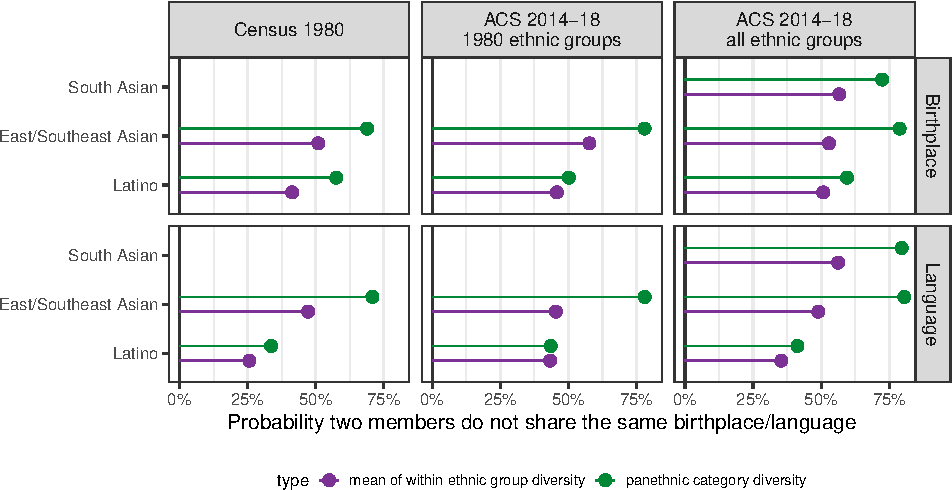
\includegraphics{main_files/figure-latex/diversity-pan-bar-1.pdf}
\caption{\label{fig:diversity-pan-bar}Birthplace and language diversity within Asian and Latino ethnic groups and panethnic categories. Diversity is measured by the Simpson diversity index which gives the probability that two randomly selected members of the group do not share the same birthplace/language. Results are based upon alternate partners from each data source. Diversity among South Asian is only measurable in the later data source due to data limitations.}
\end{figure}

Figure \ref{fig:diversity-pan-bar} shows this index for language and birthplace across East/Southeast Asian, South Asian, and Latino ethnic and panethnic categories in the two time periods. To simplify presentation, I compare the diversity across the panethnic category to the mean diversity within each specific ethnic group (weighted by group size). The likelihood of panethnic intermarriage will be reduced in cases where panethnic diversity is greater than average diversity within ethnic groups.

Significant language and birthplace diversity is observable within specific ethnic groups. For example, the average diversity in birthplace within specific Latino ethnic groups in the full ACS data is about 50\%, indicating that two randomly determined members of the same Latino ethnic group (e.g.~Mexican, Colombian) would not share the same birthplace about 50\% of the time.

Although within ethnic group diversity is substantial, panethnic diversity in language and birthplace is greater than within ethnic group diversity for all three panethnic categories in both time periods. However, these differences are small for Latinos, while they are quite large for Asians. What differences exist among Latino ethnic groups have also diminished over time, whereas they have grown for East/Southeast Asians.

Overall, Figure \ref{fig:diversity-pan-bar} shows that language and birthplace endogamy are important barriers to panethnic intermarriage among Asians, but not among Latinos. Ideally, to estimate the underlying affinity for panethnic intermarriage, we want a model that can account for language and birthplace endogamy. Such a model indicates how much panethnic intermarriage we would expect in a situation in which all Asians and Latinos are fully acculturated to the US (i.e.~born in the US and speak English as their primary language).

\hypertarget{other-methodological-limitations-of-prior-work}{%
\subsection{Other Methodological Limitations of Prior Work}\label{other-methodological-limitations-of-prior-work}}

Research on panethnic intermarriage has suffered from methodological difficulties, driven primarily by limitations in data and model design. The two primary issues have been adjusting for group size differences in local marriage markets and accounting for the issue of immigrants born abroad.

All of the studies cited above use log-linear models to adjust for differences in group size. This approach allows researchers to better estimate the underlying affinity between groups, apart from differential exposure to potential partners due to group size. However, differences in spatial settlement patterns among groups may still affect estimates in such models. Most individuals will find a partner within a local, rather than a national, context, and ethnoracial groups are not evenly distributed across the US. Without adjusting for these geographic differences, researchers will underestimate ethnoracial exogamy \citep{harris_how_2005}. This issue is particularly problematic when studying panethnicity, because Asian and Latino ethnic groups have historically settled in different parts of the US \citep{massey_geographic_2008}. Some of the prior work on panethnicity attempts to partially address this issue. \citet{fu_how_2007a} includes Census division as a parameter in log-linear models, but this regional identifier is still a very crude measure of local marriage markets. \citet{rosenfeld_salience_2001}, alternatively, estimates models separately within a few specific metropolitan areas which limits the results to the few cities with large enough samples of Asian and Latino ethnic groups to facilitate an analysis.

Because most Census data sources lack information on marriage timing, researchers have not been able to fully remove immigrants married abroad (IMA) from analysis. Because IMA were mostly married in their country of origin, their inclusion will bias estimates toward ethnic endogamy \citep{hwang_problem_1990}. Researchers have used a variety of sample restrictions to minimize this problem, but without information on marriage and migration timing, it cannot be fully eliminated.

In the analysis that follows, I address many of these prior weaknesses using a conditional logit model to estimate the likelihood of panethnic intermarriage. The data from Census 1980 and the American Community Survey 2014-18 both provide information on marriage timing which allows me to limit analysis to recent marriages while removing immigrants married abroad. The model framework also allows me to account for differences in group size in local marriage markets. Due to the model framework, I can also easily incorporate controls for birthplace and language endogamy to determine the effect these factors have on the likelihood of panethnic intermarriage.

Because of the expanded number of ethnic groups provided in the recent American Community Survey, I am able to estimate panethnic intermarriage across a more diverse set of ethnic groups than prior work. Notably, I am also able to include multiple South Asian ethnic groups into the analysis. I utilize these features to help resolve research questions about the relative magnitude of and change in panethnic intermarriage among East/Southeast Asians, South Asians, and Latinos.

\hypertarget{data-and-methods}{%
\section{Data and Methods}\label{data-and-methods}}

The data for this analysis are derived from the microdata sample of the 1980 US Census and the American Community Survey (ACS) pooled across a five year period from 2014-2018. The ACS is an annual 1-in-100 survey of the United States population, conducted by the United States Census Bureau. The 1980 US Census is the last Census dataset to include information about marriage timing, before it was re-included on the 2008 ACS. Both data sources were extracted from the Integrated Public Use Microdata Series (IPUMS) system \citep{ruggles_ipums_2020}.

In both data sources, I restrict the analysis to all opposite-sex marriages formed in the previous five years that were a first marriage for both partners. This restriction is necessary for comparison because the Census 1980 only recorded marriage timing relative to first marriage and does not include same-sex unions. To avoid including marriages occurring in a different marriage market, I also remove marriages in which at least one of the partners migrated to the US or across state lines in the last five years.

To measure the likelihood of panethnic intermarriage, I use a modeling technique that compares actual marriages to alternate marriages that were not formed \citep{gullickson_counterfactual_2021}. For each marriage, I construct a choice set of one real union and twenty fictional unions. Fictional unions are created by sampling alternate partners for one randomly determined spouse from a pool of potential partners. I then use a conditional logit model to predict how partner characteristics influence the likelihood of observing the true union, as follows: \[P_{ij}=\frac{e^{\mathbf{x}_{ij}\beta}}{\sum_{k=1}^J e^{\mathbf{x}_{ik}\beta}}\] where \(P_{ij}\) is the probability that union \(j\) within choice set \(i\) is the actual union. \(J\) is the total number of unions in the choice set. The vector \(\mathbf{x}_{ij}\) defines the characteristics of the union and the \(\beta\) vector provides estimated log-odds ratios indicating how the odds of an actual union change with \(\mathbf{x}_{ij}\). The model is estimated as a fixed-effects logistic regression model with fixed effects for each choice set.

This approach has been used previously to examine patterns of intermarriage \citep{dalmia_empirical_2001, jepsen_empirical_2002, nielsen_educational_2009, qian_marriage_2018} and friendship choices \citep{zeng_preference_2008}. This model specification has several advantages over log-linear models. Like a log-linear model, this model intrinsically accounts for differences in group size through the sampling procedure, but also takes into account the unmarried population which is ignored in a log-linear model. Furthermore, the linear structure of the conditional logit model can more easily accommodate a variety of quantitative and categorical control variables.

Arguably, the most important advantage of this modeling approach is that the researcher can specify additional restrictions in the sampling of potential partners. I utilize that feature to restrict potential partners to a locally defined marriage market, which addresses the issue of spatial dissimilarity among ethnoracial groups. Ideally, I would use metropolitan area to identify marriage markets, but not all metropolitan areas are identifiable in the public use Census 1980 and ACS data, due to confidentiality concerns. Furthermore, some respondents do not live in metropolitan areas. Therefore, I use metropolitan area as the marriage market identifier for individuals where it can be identified and otherwise I use the state of residence.\footnote{Metropolitan area is determined by IPUMS based on the county group geography in Census 1980 and the Public Use Microdata Area (PUMA) geography in the ACS. IPUMS only identifies metropolitan areas in cases where this geographic identifier unambiguously indicates residence within the metropolitan area.} I identify 255 metropolitan areas in Census 1980 and 260 metropolitan areas in the ACS data. Although I am not able to identify all metropolitan areas, most major metropolitan areas are identified in both data sources.\footnote{Because the identified metropolitan areas are not identical across time periods, some bias may be present when analyzing change over time. To address this issue, I conducted a sensitivity test using state as the marriage market for all respondents. The results for this sensitivity analysis, available in the supplementary materials, are substantively very similar to those shown here.} From within a given marriage market, I draw alternate partners from among all unmarried adults as well as individuals who were married in the previous five years, with the restriction that all alternate partners must not have migrated to the US or across state lines in the last five years.

Because this approach relies upon a random sample of alternate partners, results will vary each time this sampling procedure is performed. To account for this added uncertainty, I conduct the analysis using three different analytical samples. I then pool \(\beta\) estimates and standard errors for parallel models using the same methods as those employed for multiple imputation \citep{rubin_multiple_1987, gullickson_counterfactual_2021}.

\hypertarget{measuring-ethnoracial-exogamy}{%
\subsection{Measuring Ethnoracial Exogamy}\label{measuring-ethnoracial-exogamy}}

I measure ethnoracial categories by a combination of the race and Hispanicity questions in both data sources. Table \ref{tab:sample-size-table} shows the sample size for all ethnoracial groups included in the analysis. I classify non-Asian and non-Latino respondents as White, Black, or American Indian/Alaska Native (AIAN). Due to small sample size, I exclude Pacific Islanders, multiracial respondents, and non-Latino others. The race question includes several Asian nationalities (e.g.~Chinese, Korean, Filipino) as well as a write-in response for ethnic/national identities not captured by the existing categories. Similarly, the Hispanicity question includes major Latino ethnic groups (e.g.~Mexican, Puerto Rican, Cuban) as well as a write-in option. As indicated in Table \ref{tab:sample-size-table}, the Census 1980 data includes a far more limited set of identifiable ethnic groups for both Asians and Latinos than the ACS data. To address this restriction, I estimate two different kinds of models for the ACS data. First, I restrict the data only to those ethnic groups that were available in the Census 1980 data to allow for direct comparison over time. I then estimate models using the full set of ethnic groups available in the ACS data.

Table \ref{tab:sample-size-table} also shows how I define panethnic groups of East/Southeast Asian, South Asian, and Latino. I separate Asians into two separate panethnic blocs because prior work suggests social distance between these groups \citep{kibria_not_1996, morning_racial_2001, schachter_finding_2014}. I estimate the likelihood of intermarriage between these two blocs in all models to test whether this separation is justified empirically. Because Asian Indians are the only identifiable South Asian ethnic group in Census 1980, I cannot estimate panethnic parameters over time for South Asians. Thus, when analyzing change over time, I focus exclusively on East/Southeast Asians and Latinos.

\begin{table}

\caption{\label{tab:sample-size-table}Sample size of marriages and alternate partners by data source and ethnoracial category.}
\centering
\begin{tabu} to \linewidth {>{\raggedright\arraybackslash}p{6.5cm}>{\raggedleft}X>{\raggedleft}X}
\toprule
Category & Census 1980 & ACS 2014-2018\\
\midrule
\addlinespace[0.3em]
\multicolumn{3}{l}{\textbf{Marriages}}\\
\hspace{1em}Marriages in the previous five years & 285,523 & 503,348\\
\addlinespace[0.3em]
\multicolumn{3}{l}{\textbf{Alternate Partners}}\\
\hspace{1em}White & 2,926,629 & 4,368,640\\
\hspace{1em}Black & 535,993 & 887,837\\
\hspace{1em}American Indian/Alaska Native & 24,304 & 73,760\\
\hspace{1em}Latino & 162,526 & 859,250\\
\hspace{1em}\hspace{1em}Mexican & 113,648 & 560,124\\
\hspace{1em}\hspace{1em}Puerto Rican & 35,444 & 97,695\\
\hspace{1em}\hspace{1em}Cuban & 13,434 & 39,473\\
\hspace{1em}\hspace{1em}Salvadorian &  & 32,947\\
\hspace{1em}\hspace{1em}Dominican &  & 29,201\\
\hspace{1em}\hspace{1em}Guatemalan &  & 19,449\\
\hspace{1em}\hspace{1em}Colombian &  & 18,826\\
\hspace{1em}\hspace{1em}Honduran &  & 11,926\\
\hspace{1em}\hspace{1em}Peruvian &  & 10,548\\
\hspace{1em}\hspace{1em}Ecuadorian &  & 10,226\\
\hspace{1em}\hspace{1em}Nicaraguan &  & 7,605\\
\hspace{1em}\hspace{1em}Argentinian &  & 4,619\\
\hspace{1em}\hspace{1em}Venezuelan &  & 4,404\\
\hspace{1em}\hspace{1em}Panamanian &  & 3,960\\
\hspace{1em}\hspace{1em}Chilean &  & 2,531\\
\hspace{1em}\hspace{1em}Costa Rican &  & 2,399\\
\hspace{1em}\hspace{1em}Bolivian &  & 1,814\\
\hspace{1em}\hspace{1em}Uruguayan &  & 1,046\\
\hspace{1em}\hspace{1em}Paraguayan &  & 457\\
\hspace{1em}East and Southeast Asian & 30,432 & 199,180\\
\hspace{1em}\hspace{1em}Chinese & 9,980 & 63,621\\
\hspace{1em}\hspace{1em}Filipino & 6,557 & 48,254\\
\hspace{1em}\hspace{1em}Vietnamese & 331 & 29,119\\
\hspace{1em}\hspace{1em}Korean & 2,066 & 24,163\\
\hspace{1em}\hspace{1em}Japanese & 11,498 & 15,023\\
\hspace{1em}\hspace{1em}Cambodian &  & 4,880\\
\hspace{1em}\hspace{1em}Hmong &  & 4,563\\
\hspace{1em}\hspace{1em}Laotian &  & 3,762\\
\hspace{1em}\hspace{1em}Thai &  & 3,429\\
\hspace{1em}\hspace{1em}Burmese &  & 1,156\\
\hspace{1em}\hspace{1em}Indonesian &  & 980\\
\hspace{1em}\hspace{1em}Malaysian &  & 230\\
\hspace{1em}South Asian & 2,882 & 41,222\\
\hspace{1em}\hspace{1em}Asian Indian & 2,882 & 34,446\\
\hspace{1em}\hspace{1em}Pakistani &  & 4,785\\
\hspace{1em}\hspace{1em}Bangladeshi &  & 1,402\\
\hspace{1em}\hspace{1em}Sri Lankan &  & 589\\
\bottomrule
\end{tabu}
\end{table}

I measure patterns of ethnoracial exogamy, including panethnic intermarriage, with a set of gender-symmetric dummy variables where the reference category is an ethnoracially endogamous union (e.g.~a White-White or Chinese-Chinese marriage). Although substantial gender asymmetry exists in intermarriage for several important combinations \citep{xie_demographic_2000, gullickson_black_2006}, the use of gender-symmetric terms more closely matches my goal of estimating social boundaries between groups. Such social boundaries are best measured by averaging across gender combinations. Furthermore, given the large number of parameters involved in some models, gender asymmetric terms would be impossible to fit in many cases.

Even using gender-symmetric terms, the least parsimonious model would simply include every possible combination of categories resulting in 703 separate dummy variables in the ACS data. The sheer number of variables required and resulting data sparseness makes such a model unfeasible. Instead, I use two different approaches to more parsimoniously capture the likelihood of panethnic intermarriage and ethnoracial exogamy. The coding scheme for the first approach, illustrated in Table \ref{tab:block-diagram}, makes two simplifications. First, I model all ethnically exogamous unions within the same panethnic category using a single dummy variable that identifies the union as a panethnic intermarriage. For example, a Japanese-Korean union and a Chinese-Korean union would both be classified as East/Southeast Asian ethnic exogamy. This approach allows me to estimate the average likelihood of ethnic exogamy within a panethnic category, at the cost of neglecting potential heterogeneity in this likelihood between certain ethnic combinations. Second, when analyzing ethnoracial exogamy outside of panethnic groups, I use the larger panethnic categories of Latino, East/Southeast Asian, and South Asian. For example, a union between a White and Mexican person and between a White and a Guatemalan person would both be classified as Latino/White exogamy. These two simplifications reduce the number of required parameters to 17.

\begin{table}

\caption{\label{tab:block-diagram}A schematic representation of the coding of ethnoracial exogamy for simplified models, using three example ethnicities for Asian and Latino populations. The table shows a crosstabulation of each partner's race. All parameters are gender-symmetric, so I only show the parameters below the diagonal. The reference category is an ethnoracially endogamous union. Each cell indicates the particular dummy variable that is applied to a given case. The terms measuring panethnicity are shown in bold.}
\centering
\resizebox{\linewidth}{!}{
\begin{tabular}[t]{l>{}c>{}c>{}c>{}c>{}c>{}c>{}c>{}c}
\toprule
\multicolumn{3}{c}{ } & \multicolumn{3}{c}{Asian} & \multicolumn{3}{c}{Latino} \\
\cmidrule(l{3pt}r{3pt}){4-6} \cmidrule(l{3pt}r{3pt}){7-9}
  & White & Black & Chinese & Japanese & Korean & Mexican & Cuban & Puerto Rican\\
\midrule
White & \em{(ref.)} &  &  &  &  &  &  & \\
Black & B/W & \em{(ref.)} &  &  &  &  &  & \\
\addlinespace[0.3em]
\multicolumn{9}{l}{\textbf{Asian}}\\
\hspace{1em}Chinese & A/W & A/B & \em{(ref.)} &  &  &  &  & \\
\hspace{1em}Japanese & A/W & A/B & \textbf{PE-A} & \em{(ref.)} &  &  &  & \\
\hspace{1em}Korean & A/W & A/B & \textbf{PE-A} & \textbf{PE-A} & \em{(ref.)} &  &  & \\
\addlinespace[0.3em]
\multicolumn{9}{l}{\textbf{Latino}}\\
\hspace{1em}Mexican & L/W & L/B & L/A & L/A & L/A & \em{(ref.)} &  & \\
\hspace{1em}Cuban & L/W & L/B & L/A & L/A & L/A & \textbf{PE-L} & \em{(ref.)} & \\
\hspace{1em}Puerto Rican & L/W & L/B & L/A & L/A & L/A & \textbf{PE-L} & \textbf{PE-L} & \em{(ref.)}\\
\bottomrule
\multicolumn{9}{l}{\rule{0pt}{1em}\textit{Notes: }}\\
\multicolumn{9}{l}{\rule{0pt}{1em}B/W=Black/White, A/W=Asian/White, A/B=Asian/Black, L/W=Latino/White, L/B=Latino/Black,}\\
\multicolumn{9}{l}{\rule{0pt}{1em}L/A=Latino/Asian, PE-A=Panethnic Asian, PE-L=Panethnic Latino}\\
\end{tabular}}
\end{table}

This approach may miss important heterogeneity in the likelihood of ethnoracial exogamy. To address this issue, I also fit a less parsimonious model to the ACS data, in which I use a separate dummy variable for each specific combination of ethnic groups within the same panethnic category. Additionally, to determine whether the tendency to outmarry with Whites or Blacks varies among ethnic groups within the same panethnic category, I treat each combination of an ethnic group with the White and Black categories as a separate variable. I restrict the ethnic groups to those for which I can fit a model without problems of sparseness and model non-convergence, determined by sequentially including ethnic groups by size. The final model includes the five East/Southeast Asian ethnic groups available in the Census 1980 data (Chinese, Filipino, Vietnamese, Korean, and Japanese) and the ten largest Latino groups, with the exception of Hondurans. I could not fit these models for South Asians because of the small size of non-Asian Indian groups in the South Asian category. This model includes 85 separate exogamy terms that better capture heterogeneity within panethnic categories but at a significant cost to parsimony.

Regardless of the specific model, the exponentiated coefficient for each ethnoracial exogamy term can be interpreted as the ratio of the odds of a union between the two specified ethnoracial groups relative to the odds of ethnoracial endogamy. Values below one indicate that exogamy is less likely than endogamy. A relatively lower odds ratio indicates lower likelihood of this form of exogamy relative to other forms of exogamy. These odds ratios represent the likelihood of intermarriage net of group size differences in partner availability. These group size differences are accounted for by the sampling procedure which will draw alternate partners from different groups in proportion to their size in the designated marriage market.

Each odds ratio is also unaffected by the degree of ethnoracial exogamy to other groups. For a given focal group, a high odds ratio of exogamy to one group does not entail that the odds ratio of exogamy to other groups must necessarily be low. Theoretically, for example, the odds ratio of exogamy to all outgroups could equal one, indicating no preference for endogamy and that partnering was conducted randomly with regard to ethnorace.

\hypertarget{measuring-birthplace-and-language-endogamy}{%
\subsection{Measuring Birthplace and Language Endogamy}\label{measuring-birthplace-and-language-endogamy}}

I account for language and birthplace endogamy with simple dummy variables indicating whether the two potential partners share the same primary language or birthplace, respectively. Primary language is determined by what language the respondent reported speaking at home. Because this variable is measured after a marriage occurred, it may somewhat overestimate language endogamy among respondents.

Birthplace endogamy is complicated by the ``1.5'' generation -- individuals born outside of the United States but who migrated as children and whose formative experiences are partially defined by acculturation within the US. I consider three possibilities for coding the birthplace endogamy of such individuals. First, such individuals could be considered birthplace endogamous only with a person from the same actual birthplace. Second, such individuals could be considered birthplace endogamous with either a person from their actual birthplace or a person born in the USA. Third, such individuals could be considered only birthplace endogamous with a person born in the USA.

To test the accuracy of these three possibilities, I fit models using each coding scheme to the Census 1980 and ACS data. Following \citet{rumbaut_ages_2004a}, I also divide the 1.5 generation into a ``1.75'' generation (those who arrived in the US before the age of 6), a ``1.5'' generation (those who arrived in the US between the ages of 6-12), and a ``1.25'' generation (those who arrived in the US between the ages of 13-17). For these three groups, I consider every possible combination of coding such that earlier generations are not more acculturated than later generations. Table \ref{tab:deviance-bendog} shows the model fit by deviance of all ten possible combinations for both data sources. Lower deviance indicates better fit.

\begin{table}

\caption{\label{tab:deviance-bendog}Model fit to Census 1980 and ACS data using different specifications of birthplace endogamy for 1.25, 1.5, and 1.75 generations. Minimum deviance is shown in bold.}
\centering
\begin{tabu} to \linewidth {>{\raggedright}X>{\raggedright}X>{\raggedright}X>{\raggedleft}X>{\raggedleft}X}
\toprule
\multicolumn{3}{c}{Generation} & \multicolumn{2}{c}{Model Deviance} \\
\cmidrule(l{3pt}r{3pt}){1-3} \cmidrule(l{3pt}r{3pt}){4-5}
1.75 & 1.5 & 1.25 & Census 1980 & ACS 2014-18\\
\midrule
Birthplace & Birthplace & Birthplace & \textbf{1,122,736} & 1,850,594\\
Both & Birthplace & Birthplace & 1,122,758 & 1,849,753\\
USA & Birthplace & Birthplace & 1,122,856 & 1,850,491\\
Both & Both & Birthplace & 1,122,775 & \textbf{1,849,202}\\
USA & Both & Birthplace & 1,122,851 & 1,849,714\\
USA & USA & Birthplace & 1,123,002 & 1,851,089\\
Both & Both & Both & 1,122,932 & 1,850,676\\
USA & Both & Both & 1,122,968 & 1,850,894\\
USA & USA & Both & 1,123,013 & 1,851,576\\
USA & USA & USA & 1,122,968 & 1,852,855\\
\bottomrule
\multicolumn{5}{l}{\rule{0pt}{1em}\textit{Notes: }}\\
\multicolumn{5}{l}{\rule{0pt}{1em}Age of US arrival by generation is 0-5 (1.75), 6-12 (1.5), and 13-17 (1.25). All models include}\\
\multicolumn{5}{l}{\rule{0pt}{1em}controls for educational differences, age differences, ethnoracial endogamy, and language}\\
\multicolumn{5}{l}{\rule{0pt}{1em}endogamy.}\\
\end{tabu}
\end{table}

For both time periods, the preferred models use birthplace only coding for those respondents who entered the US after age 12. The USA only option was not preferred for any group in either time period. In the Census 1980 data, the most preferred model treats all three groups as first generation individuals. The preferred model in the ACS data treats the 1.75 and 1.5 generations as birthplace endogamous with partners either from the actual birthplace or the USA, suggesting greater acculturation of the 1.5 and 1.75 generation today than in 1980. For all subsequent models, I code birthplace endogamy according to the best-fitting model for each data source from Table \ref{tab:deviance-bendog}.

\hypertarget{additional-variables}{%
\subsection{Additional Variables}\label{additional-variables}}

All models include controls for age and educational differences between potential partners. Age differences are modeled by taking the numerical age difference between partners and its square. Educational differences are modeled using educational crossing parameters \citep{schwartz_trends_2005} with four categories of education (less than a high school diploma, a high school diploma, some college education, and at least a four-year college degree). I also include parameters that measure the likelihood of female educational hypergamy (marrying up by education) and female educational hypogamy (marrying down by education).

\hypertarget{results}{%
\section{Results}\label{results}}

I begin by illustrating results from models which use a single ethnic exogamy term for each panethnic category. I show how the strength of these ethnic exogamy terms changes with the inclusion of controls for birthplace and language endogamy, followed by an examination of how the strength of panethnicity has changed over time and in relation to other forms of ethnoracial exogamy.\footnote{The analysis of change over time relies upon two time points where the data are sufficient to identify recent marriages. It is possible that patterns of ethnoracial exogamy changed in non-linear ways in the interim between these periods.} I then move to the less parsimonious models that examine heterogeneity in panethnicity among ethnic groups belonging to the same panethnic category for the later time period.

I use graphical visualizations to present important results from all models. Results are presented as the ratio of the odds of a given form of exogamy to the odds of ethnoracial endogamy. An odds ratio of one indicates that the given form of exogamy is as likely as endogamy. Full results upon which figures are based are available in the supplementary materials.

\hypertarget{the-strength-of-panethnicity}{%
\subsection{The Strength of Panethnicity}\label{the-strength-of-panethnicity}}

Figure \ref{fig:exog-lolly} shows the estimated odds of ethnic exogamy relative to ethnic endogamy for all three panethnic categories in both time periods.

\begin{figure}
\centering
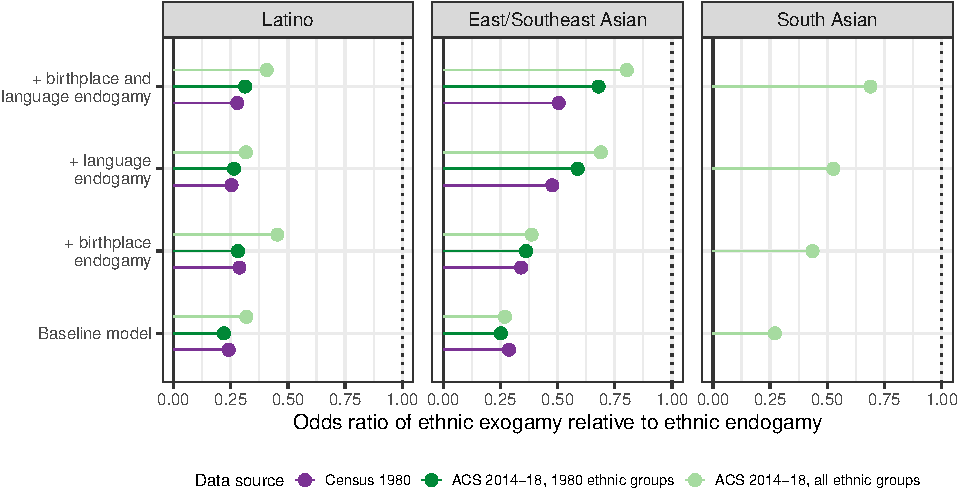
\includegraphics{main_files/figure-latex/exog-lolly-1.pdf}
\caption{\label{fig:exog-lolly}The odds of ethnic exogamy for Latinos, East/Southeast Asians, and South Asians over time and model specification. The baseline model controls for age and educational differences.}
\end{figure}

The baseline model adjusts for age and educational differences between potential partners. I then add birthplace and language endogamy separately and together to determine the effects of these variables on the odds of ethnic exogamy.

In the baseline model, the odds of ethnic exogamy are similar for all three categories. Ethnic exogamy is about 25\% as likely as ethnic endogamy. The results also show a very slight decline in the odds of ethnic exogamy from 1980 to 2014-2018 among ethnic groups identifiable in the 1980 data.

For Latinos, controlling for birthplace and language endogamy slightly increases the odds of ethnic exogamy across all models. Consistent with the results from Figure \ref{fig:diversity-pan-bar}, birthplace and language endogamy are not strong barriers to panethnic intermarriage among Latinos.

In contrast, for both Asian panethnic categories, controlling for birthplace and language endogamy substantially increases the odds of ethnic exogamy. In the ACS data, the relative odds of ethnic exogamy rise to roughly 75\% for both East/Southeast Asians and South Asians once I control for language and birthplace endogamy. Controlling for language endogamy produces larger changes than controlling for birthplace endogamy, but both variables play a role. The odds of ethnic exogamy for East/Southeast Asians also increased substantially over time in models that account for birthplace and language endogamy.

For both Latinos and East/Southeast Asians, ethnic exogamy is more likely in models that include all ethnic groups from the ACS data rather than just the groups that were available in the Census 1980 data. These results suggest greater ethnic exogamy among these more recent and smaller groups.

Figure \ref{fig:exog-lolly} shows the important role that birthplace and language endogamy play in panethnic intermarriage. In actuality, we observe similar odds of ethnic exogamy among Asians and Latinos. However, the low odds of ethnic exogamy for Asians are largely a function of the high level of diversity in birthplace and language between Asian ethnic groups. These barriers do not exist for Latinos. Controlling for these factors reveals a stronger affinity for panethnicity among Asians than Latinos.

Figure \ref{fig:changes-intermar} shows the odds of East/Southeast Asian and Latino ethnic exogamy in comparison to the odds of ethnoracial exogamy more broadly. All results in Figure \ref{fig:changes-intermar} are from the model that accounts for birthplace and language endogamy. East/Southeast Asian ethnic exogamy stands out as far more likely than any form of interracial marriage. Latino ethnic exogamy, on the other hand, does not stand out. When limiting the analysis to comparable ethnic groups over time, White-Latino intermarriage has become slightly more likely than Latino ethnic exogamy by the later time period. When the analysis is expanded to all Latino ethnic groups, Latino ethnic exogamy is only sightly more likely than White-Latino exogamy in the recent time period.

\begin{figure}
\centering
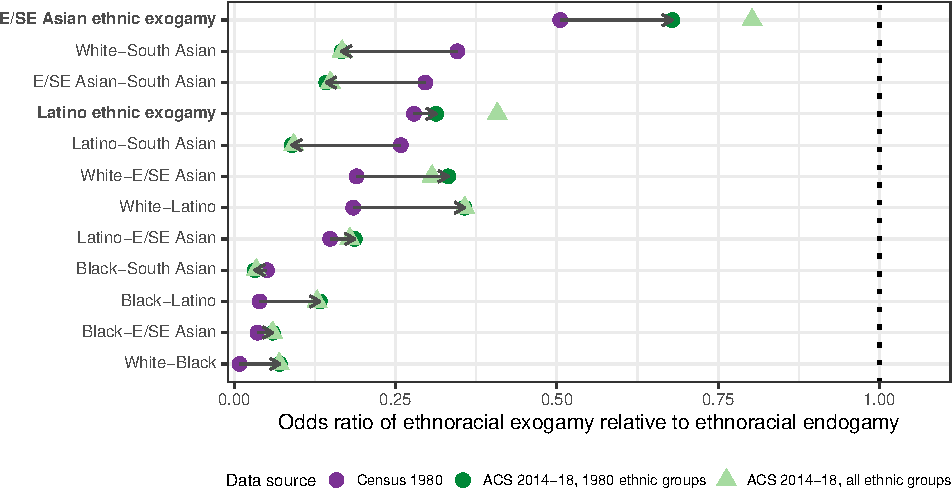
\includegraphics{main_files/figure-latex/changes-intermar-1.pdf}
\caption{\label{fig:changes-intermar}Odds of ethnoracial exogamy relative to endogamy across two time periods. Results are based on models that control for age differences, educational differences, and birthplace and language endogamy. Values are sorted by ethnoracial exogamy in 1980. Arrows show the change across the two time periods based on comparable sets of ethnic groups. Results for American Indian/Alaska Native intermarriage are excluded due to sampling variability.}
\end{figure}

Figure \ref{fig:changes-intermar} shows a relatively low odds of intermarriage between South Asians and East/Southeast Asians in both time periods. In the more recent ACS data, the odds of an East/Southeast Asian-South Asian intermarriage were only 14\% as high as the odds of ethnic endogamy, making it one of the less likely forms of intermarriage and justifying the decision to separate out these panethnic blocs empirically. The figure also shows significant declines in South Asian interracial marriage with all other groups over the time period. This finding, however, should be viewed with caution. In the earlier time period, the only South Asian group available was Asian Indian and research has shown that respondents sometimes confuse the categories of ``Asian Indian'' and ``American Indian'' in race responses \citep{liebler_american_2004}. Given the novel character of the Asian Indian category in 1980, it is likely that such misreporting has decreased over time which may contribute to the overall decline in interracial marriage over time, if American Indians are less endogamous, on average, than Asian Indians.\footnote{Although not shown here, I also found that the odds of intermarriage between American Indian/Alaska Natives and South Asians was roughly 1.9 to 1 in 1980 but declined to 0.103 to 1 in the later ACS data. This result suggests that such race reporting errors played a greater role in 1980 than the later data.}

\hypertarget{heterogeneity-in-panethnicity-across-groups}{%
\subsection{Heterogeneity in Panethnicity across Groups}\label{heterogeneity-in-panethnicity-across-groups}}

The preceding models used a single ethnic exogamy term for each panethnic category such that the odds of ethnic exogamy are assumed to be the same regardless of which specific groups are paired. I now turn to models of the ACS data that relax this assumption and fit more detailed terms between each possible pair of ethnic groups. Additionally, these models also include ethnic group specific parameters for intermarriage with Whites and Blacks. By necessity, these models are limited to the largest ethnic groups within each panethnic category.

Figure \ref{fig:ethnic-heat-map} shows the group-specific odds of ethnic exogamy for the five East/Southeast Asian ethnic groups and the nine Latino ethnic groups for which I could fit models. I also provide a dendrogram that indicates the relative distance between each of these ethnic groups, determined by treating the inverse of the odds ratio as a measure of distance and measuring unweighted average distances.

\begin{figure}
\centering
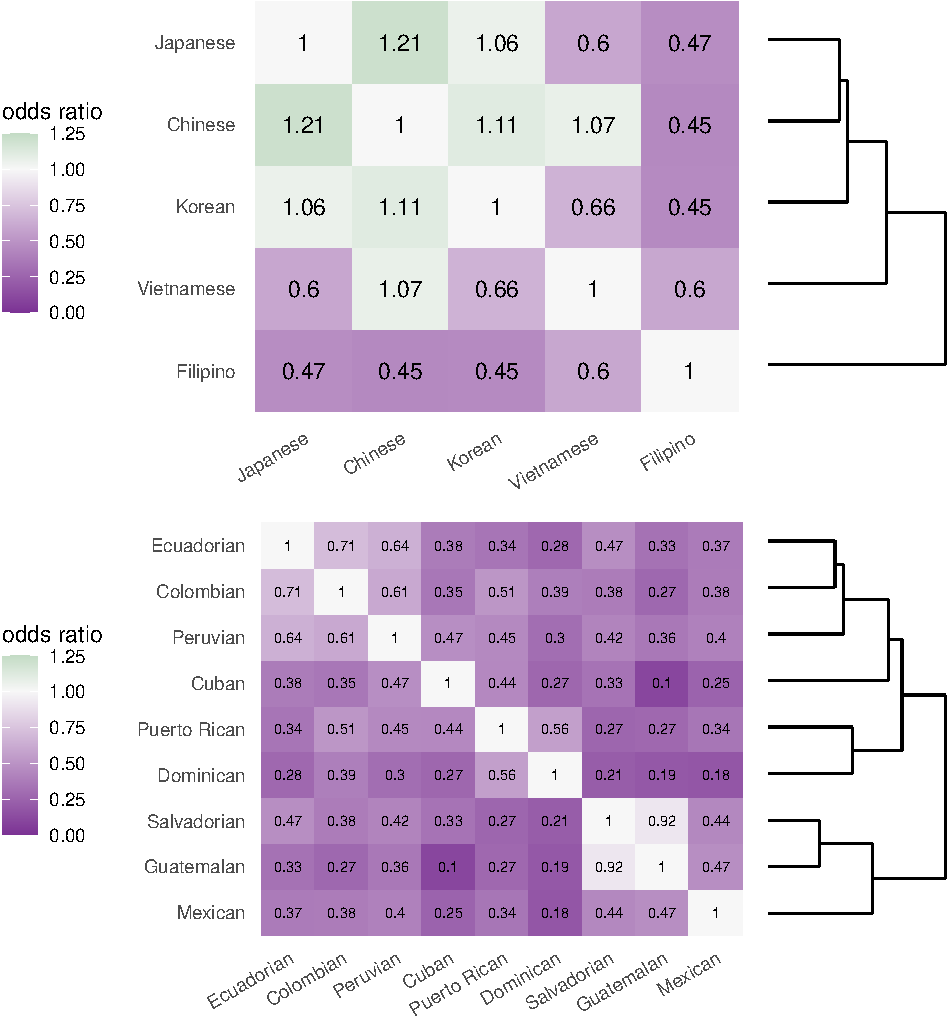
\includegraphics{main_files/figure-latex/ethnic-heat-map-1.pdf}
\caption{\label{fig:ethnic-heat-map}Odds of ethnic exogamy relative to ethnic endogamy between ethnic groups in ACS 2014-2018 data. The upper panel shows East/Southeast Asian ethnic groups and the lower panel shows Latino ethnic groups. Dendrograms on the right are based on hierarchical clustering using unweighted average distances where distance was measured by the inverse of these odds ratios. Results are based on models that control for age differences, education differences, and language and birthplace endogamy.}
\end{figure}

The top panel of Figure \ref{fig:ethnic-heat-map} shows no social distance between the three East Asian groups of Chinese, Korean, and Japanese. The point estimates suggest that, holding language and birthplace endogamy constant, the odds of ethnic exogamy are slightly higher than ethnic endogamy among these groups. However, none of these odds ratios are statistically distinguishable from one at \(p<.05\).

Social distance remains between these East Asian groups and the Vietnamese and Filipino ethnic groups, with the exception of the Vietnamese-Chinese case for which there is no barrier to ethnic exogamy. These results indicate some regional distinction in panethnic intermarriage among East/Southeast Asians. Filipinos, in particular, have the lowest odds of ethnic exogamy with all of the other Asian groups, suggesting a stronger boundary separating Filipinos from wider East/Southeast Asian panethnicity, which may reflect the unique Spanish cultural inheritance of the Philippines. To test this hypothesis, I included a dummy variable for Latino-Filipino intermarriage and found that the odds of this form of intermarriage were about double those between Latinos and other East/Southeast Asian groups.

The bottom panel of Figure \ref{fig:ethnic-heat-map} shows comparable results for the nine Latino ethnic groups. Overall, the odds ratios are much lower than for Asian ethnic groups, reflecting the overall lower ethnic exogamy among Latinos. Salvadorian-Guatemalan intermarriage was the only case with little evidence of social distance.

Affinities between Latino ethnic groups tend to cluster by region, with higher odds of intermarriage within the three groups of South American, Caribbean, and Central American/Mexican nationalities. The one exception to this pattern is for Cubans, who tend to be about equal distance from both the South American and Caribbean groupings.

Figure \ref{fig:racial-exogamy} shows the odds of intermarriage with Whites and Blacks for each of the East/Southeast Asian and Latino ethnic groups. For comparison, the ethnic exogamy odds ratios for a given ethnic group are also shown with small grey dots.

\begin{figure}
\centering
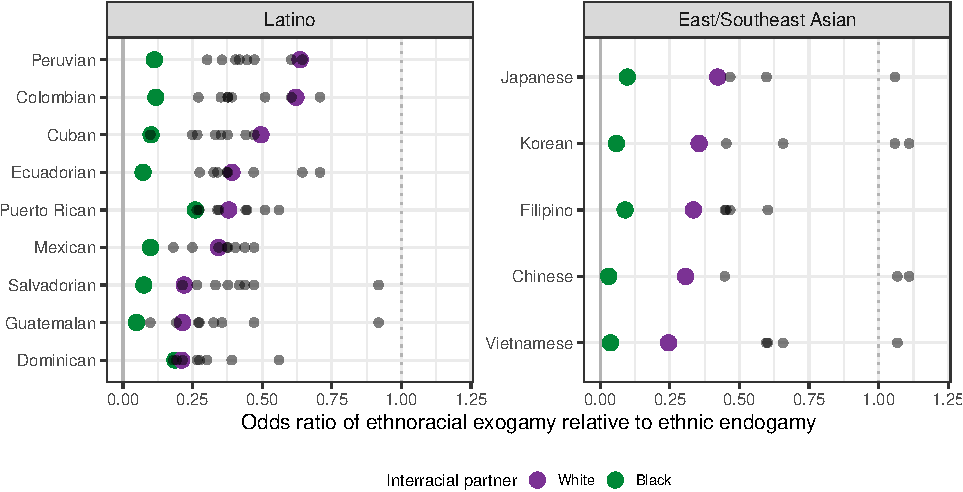
\includegraphics{main_files/figure-latex/racial-exogamy-1.pdf}
\caption{\label{fig:racial-exogamy}Odds of exogamy with Whites and Blacks for major Latino and East/Southeast Asian ethnic groups. For reference, odds of ethnic exogamy to major ethnic groups within the same category are shown by small grey dots. Groups are sorted based on the odds ratio of exogamy with Whites. All models control for age differences, education differences, and language and birthplace endogamy.}
\end{figure}

Variation in the likelihood of interracial marriage across ethnic groups is more pronounced for Latino ethnic groups than for East/Southeast Asian groups. Among Latinos, Peruvians and Colombians are the most likely to intermarry with Whites with an odds about 60\% as high as ethnic endogamy. At the other end of the spectrum, the odds ratio of Dominican-White intermarriage is just under 25\%. For the five East/Southeast Asian groups, the odds ratios range from 25\% to 42\%.

For all East/Southeast Asian and Latino ethnic groups, intermarriage with Whites is more likely than intermarriage with Blacks. The odds of intermarriage with Blacks are uniformly low for all five East/Southeast Asian groups. The odds of intermarriage are also low for most Latino groups, with the exception of Dominicans and Puerto Ricans. For Dominicans, the odds of intermarriage with Blacks are almost identical to the odds of intermarriage with Whites. For Puerto Ricans, the odds of intermarriage with Blacks are the highest of any Latino ethnic group and only slightly less likely than the odds of intermarriage with Whites.

The relative placement of ethnic exogamy odds ratios for each ethnic group in Figure \ref{fig:racial-exogamy} is also telling. For all five Asian ethnic groups, every ethnic exogamy parameter is greater than the odds of intermarriage with Whites. For the Latino groups, these ethnic exogamy parameters are frequently in-between the odds of White and Black intermarriage. For example, both Peruvians and Cubans are more likely to outmarry to a white person than to intermarry with any of the other Latino groups. Mexicans are only slightly more likely to outmarry to most other Latino ethnic groups as they are to outmarry with whites, and are substantially less likely in two cases (Dominicans and Cubans).

Overall, Figure \ref{fig:racial-exogamy} implies very different patterns of intermarriage for Latino and East/Southeast Asian ethnic groups. East/Southeast Asian ethnic groups follow the same general pattern. Panethnic intermarriage is more likely than intermarriage with Whites or Blacks, and the barriers to intermarriage with Blacks are far more substantial than the barriers to intermarriage with Whites. Furthermore the likelihood of intermarriage with Whites and Blacks is relatively similar across ethnic groups. The consistency of this pattern speaks to a broad panethnic pattern of intermarriage for East/Southeast Asians, even given some regional and national variation.

On the other hand, the results for Latino groups are characterized by ethnic-specific heterogeneity. In no case is ethnic exogamy clearly preferred to outmarriage with Whites and there are large differences across ethnic groups in the tendency to intermarry with both Whites and Blacks. These results are not consistent with a singular pattern of intermarriage, panethnic or otherwise, among Latinos.

\hypertarget{conclusions}{%
\section{Conclusions}\label{conclusions}}

This article analyzed the evidence for panethnicity in the partner choices that individuals make in marriage. What evidence do I find for panethnic intermarriage among Asians and Latinos and has this tendency changed over time?

Answering this question is complicated by the diversity of birthplace and language among and within Asian and Latino ethnic groups due to continuing immigration from abroad. Theoretically, such diversity could affect panethnic intermarriage in different ways depending on whether it is greater between rather than within ethnic groups belonging to the same panethnic category. In actuality, it serves as a barrier to panethnic intermarriage among Asians, but not Latinos.

Accounting for birthplace and language endogamy, I find strong affinity between East/Southeast Asian ethnic groups and between South Asian ethnic groups, respectively. In both cases, the odds of ethnic exogamy are about 75\% as high as the odds of ethnic endogamy in the more recent 2014-2018 ACS data. In the case of East/Southeast Asians, I can show that panethnic affinity has grown over time. The odds of ethnic exogamy among Asians are also much higher than the odds of any form of interracial outmarriage.

I find no evidence of panethnic affinity between East/Southeast Asians and South Asians. Scholars have raised the question of whether panethnic Asian coalitions in the US truly include South Asians \citep{kibria_not_1996}. In terms of the interpersonal panethnicity measured here, the answer is a resounding no. What emerges instead are two distinct ``melting pots'' of panethnic affinity among Asian populations.

I find much weaker affinity among Latino ethnic groups. Even after controlling for birthplace and language endogamy, the odds of ethnic exogamy are only about 25\% as high as the odds of ethnic endogamy in both time periods. These odds are quite similar to the odds of Latino-White intermarriage, suggesting that relative to other forms of exogamy, panethnic intermarriage is not a strong force.

In the ACS data, I am able to include a wide variety of ethnic groups and find that when I use more groups, the odds of ethnic exogamy are slightly higher for both East/Southeast Asians and Latinos. I also examine more specific affinities among ethnic groups within the same panethnic category. The results support the more general conclusions, but show some tendency towards regional affinities in both cases. I also find greater heterogeneity in the intermarriage patterns of Latinos by ethnicity.

The results here help to resolve ambiguous findings regarding the strength of panethnicity among Latinos. I find much weaker evidence of panethnic affinity in marriage among Latinos than among Asians. Why is panethnic affinity stronger among Asian ethnic groups than among Latino ethnic groups? Consistent with prior research, the results here suggest the relative importance of the structural rather than cultural factors that encourage panethnicity \citep{lopez_panethnicity_1990}. Specifically, Asians (and in particular East/Southeast Asians) are more likely than Latinos to be racialized due to more phenotype similarity and a broad panethnic ``model minority'' stereotype \citep{lopez_panethnicity_1990, kibria_construction_1997, rosenfeld_salience_2001}. My results are consistent with that argument and suggest that racialization also affects this most interpersonal form of panethnicity. This is not to say that racialization plays no role for Latinos, but rather due to greater phenotype diversity as well as other structural differences, the racialization of Latinos has been more contested \citep{rodriguez_changing_2000a, frank_latino_2010a, fox_defining_2013}.

Scholars often treat intermarriage not only as a direct measure of social distance between groups but also as a mechanism for the further breakdown of barriers between groups, because intermarriage will generated progeny of mixed identification in the next generation \citep{gordon_assimilation_1964}. However, group size complicates any attempt to analyze these features of intermarriage simultaneously. I use models that remove the issue of group size from consideration when estimating the odds of ethnoracial intermarriage. Such models do a better job at estimating the underlying affinity between groups, but the actual frequency of interethnic and interracial marriages will depend much more heavily on group size. For example, because Asian ethnic groups tend to be small within the larger US population, the actual frequency of Asian-White intermarriages will likely be more common than interethnic marriages among Asians, even if Asian individuals prefer the latter type of union. This issue complicates our understanding of how the growth of interethnically married couples and their progeny will affect future racial boundaries.

Understanding the future is further complicated by continuing migration to the US. The strong panethnic affinity I observe among East/Southeast Asian and South Asian ethnic groups only emerges net of the strong tendency toward birthplace and language endogamy. In a situation in which all members of these groups are English-speaking native-born individuals, we would expect such affinities to emerge. In actuality, such affinities are suppressed by the high birthplace and language diversity resulting from continued migration. The future strength of panethnic intermarriage depends very much on future patterns of immigration.



\renewcommand\refname{References}
\bibliography{../project.bib}
\end{document}

\processdelayedfloats
